\documentclass[11pt,a4paper]{article}
\usepackage[T1]{fontenc}
\usepackage[utf8]{inputenc}
\usepackage[french]{babel}
\usepackage[margin=2.2cm]{geometry}
\usepackage{amsmath}
\usepackage{booktabs}
\usepackage{graphicx}
\usepackage{caption}
\usepackage{float}
\usepackage{pgfplots}
\pgfplotsset{compat=1.16}
\usepackage[hidelinks]{hyperref}

\title{Analyse modale d'une roue aubagée\\[2pt]
\large Effet du raidissement centrifuge (\emph{stress stiffening})}
\author{}
\date{12 novembre 2026}

\begin{document}
\maketitle
\vspace{-3.5em}

\paragraph{Résumé.}
Les vingt premiers modes d'une roue aubagée monobloc de 20 pales sont calculés
avec code\_aster, à l'arrêt puis à 10\,000~tr/min en ajoutant la raideur
géométrique due à la précontrainte centrifuge. Le raidissement relève les
fréquences de 5,3 à 6,5~\%, en accord avec la loi de Southwell.
L'assouplissement centrifuge n'est pas inclus dans ce calcul.

\section{Modèle}

\begin{minipage}[c]{0.50\textwidth}
\begin{itemize}\setlength\itemsep{1pt}
\item Roue complète 360°, disque et pales monoblocs, axe de rotation $Z$ ;
      alésage $R=40$~mm, pied de pale $R=150$~mm, hauteur de pale 60~mm.
\item Maillage conforme de 289\,440 HEXA8 (316\,481 n\oe uds, 919\,440 degrés
      de liberté actifs), généré par \texttt{roue\_aubagee.py}.
\item Matériau TA6V : $E=110$~GPa, $\nu=0{,}31$, $\rho=4430$~kg/m$^3$.
\item Un n\oe ud \texttt{CENTRE} placé sur l'axe porte 6 degrés de liberté
      (élément discret). Il est lié rigidement à l'alésage
      (\texttt{LIAISON\_SOLIDE}) puis encastré.
\item La rotation est un chargement volumique centrifuge
      (\texttt{ROTATION}, $\Omega = 1047$~rad/s autour de $Z^+$).
\end{itemize}
\end{minipage}\hfill
\begin{minipage}[c]{0.46\textwidth}
\centering
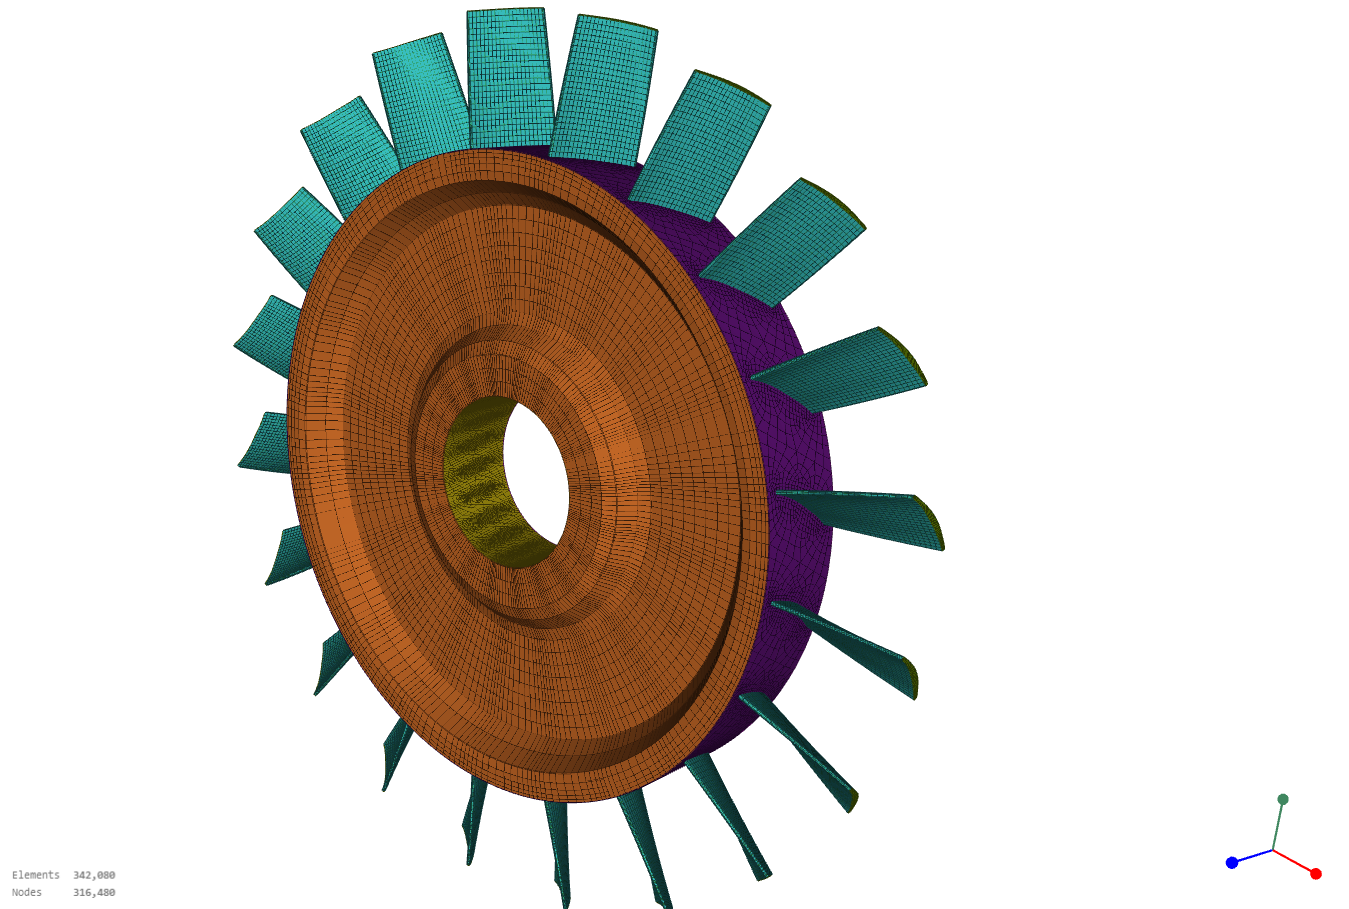
\includegraphics[width=\linewidth,trim=220 0 380 0,clip]{maillage.png}
\captionof{figure}{Maillage de la roue.}
\end{minipage}

\section{Méthode}

Un calcul statique linéaire sous chargement centrifuge fournit le champ de
contraintes $\sigma_0$. On en déduit la matrice de raideur géométrique
$K_g(\sigma_0)$, puis on résout deux problèmes aux valeurs propres :
\begin{align*}
\text{à l'arrêt :}\quad & \bigl(K - \omega^2 M\bigr)\,\phi = 0, \\
\text{en rotation :}\quad & \bigl(K + K_g(\sigma_0) - \omega^2 M\bigr)\,\phi = 0.
\end{align*}
Les 20 plus petites fréquences sont extraites dans chaque cas
(\texttt{CALC\_MODES}, méthode de Sorensen). La norme d'erreur moyenne des
modes est de l'ordre de $10^{-9}$.

\section{Résultats}

\begin{table}[H]
\centering
\begin{tabular}{lccc}
\toprule
Modes & À l'arrêt (Hz) & En rotation (Hz) & Écart \\
\midrule
1--2 (doublet)  & 963,8  & 1014,6 & $+5{,}3$~\% \\
3 (simple)      & 988,0  & 1046,2 & $+5{,}9$~\% \\
4--5 (doublet)  & 992,6  & 1053,4 & $+6{,}1$~\% \\
6--7 (doublet)  & 1022,3 & 1088,8 & $+6{,}5$~\% \\
8--19 (doublets) & 1026,5 à 1028,5 & 1093,4 à 1095,6 & $+6{,}5$~\% \\
20 (simple)     & 1028,5 & 1095,6 & $+6{,}5$~\% \\
\bottomrule
\end{tabular}
\caption{Fréquences propres à l'arrêt et à 10\,000~tr/min, comparées par rang.}
\end{table}

\begin{figure}[H]
\centering
\begin{tikzpicture}
\begin{axis}[width=0.78\textwidth, height=5.6cm,
  xlabel={Rang du mode}, ylabel={Fréquence (Hz)},
  xmin=0, xmax=21, ymin=940, ymax=1120,
  grid=major, grid style={gray!25},
  yticklabel style={/pgf/number format/1000 sep={}},
  legend pos=south east, legend cell align=left]
\addplot[mark=*, mark size=1.6pt, blue!70!black] coordinates {
(1,963.813)(2,963.813)(3,988.031)(4,992.593)(5,992.593)(6,1022.348)
(7,1022.348)(8,1026.521)(9,1026.521)(10,1027.669)(11,1027.669)(12,1028.117)
(13,1028.117)(14,1028.327)(15,1028.327)(16,1028.432)(17,1028.432)
(18,1028.483)(19,1028.483)(20,1028.499)};
\addplot[mark=square*, mark size=1.6pt, red!75!black] coordinates {
(1,1014.551)(2,1014.551)(3,1046.220)(4,1053.401)(5,1053.401)(6,1088.780)
(7,1088.780)(8,1093.430)(9,1093.430)(10,1094.692)(11,1094.692)(12,1095.182)
(13,1095.182)(14,1095.411)(15,1095.411)(16,1095.526)(17,1095.526)
(18,1095.582)(19,1095.582)(20,1095.599)};
\legend{À l'arrêt ($K$), En rotation ($K+K_g$)}
\end{axis}
\end{tikzpicture}
\caption{Les 20 premières fréquences propres dans les deux configurations.}
\end{figure}

\paragraph{Structure des modes.}
Les 20 modes se répartissent en 9 doublets et 2 modes simples : c'est une
famille complète d'une roue à 20 pales (diamètres nodaux 0 à 10). Les
fréquences s'accumulent vers 1028~Hz (1096~Hz en rotation), fréquence à
laquelle le disque ne participe plus au mouvement. Il s'agit
vraisemblablement de la première flexion de pale ; les déformées n'ont pas
été examinées.

\paragraph{Cohérence avec la loi de Southwell.}
Cette loi s'écrit $f^2 = f_0^2 + S\,\Omega^2$, avec ici
$\Omega = 166{,}7$~Hz. Le dernier mode donne
\[
S = \frac{1095{,}6^2 - 1028{,}5^2}{166{,}7^2} \approx 5{,}1 .
\]
Pour la première flexion d'une poutre encastrée uniforme montée sur un moyeu,
le coefficient vaut environ $1{,}2 + 1{,}6\,R_\text{pied}/L$, soit environ 5
pour $R_\text{pied}/L = 2{,}5$. L'ordre de grandeur est donc le bon ; la pale
réelle étant vrillée et effilée, ce recoupement n'est pas une validation fine.

\section{Limites}
\begin{itemize}\setlength\itemsep{1pt}
\item L'assouplissement centrifuge (\texttt{RIGI\_ROTA}) n'est pas inclus :
      les fréquences en rotation sont légèrement surestimées. Il s'active
      avec \texttt{ASSOUPLISSEMENT = True} dans \texttt{modal\_roue.comm}.
\item Les effets gyroscopiques (Coriolis) sont négligés.
\item La précontrainte vient d'un calcul statique linéaire, et la liaison
      rigide empêche l'alésage de se dilater (variante \texttt{RBE3}
      disponible dans le fichier de commandes).
\item Les modes sont comparés par rang, sans appariement des déformées.
\end{itemize}

\end{document}
